\documentclass[UTF8]{book}
\usepackage{graphicx}
\usepackage{amsmath}
\usepackage{amsfonts}
\usepackage{amssymb}
\usepackage{geometry}
\usepackage{float}
\geometry{a4paper,scale=0.8}
\usepackage{listings}
\lstset{
	basicstyle=\sffamily,
	keywordstyle=\bfseries,
	commentstyle=\rmfamily\itshape,
	stringstyle=\ttfamily}
\newcommand{\iocode}[2]{\lstinline[language=Mathematica]|#1|\hspace{\fill}\emph{Output:#2}}
\newcommand{\incode}[1]{\lstinline[language=Mathematica]|#1|}
\begin{document}
	\sffamily
	\author{Hu Xiping}
	\title{Note on Mathematica Programming}
	\date{\today}
	\maketitle
	\tableofcontents
	\part{Basics of Wolfram Language}
		\chapter{Features of Mathematica}
			\section{Evaluating Commands}
				On desktop and web, you may press \textbf{Shift}+\textbf{Enter}. On mobile, press the Wolfram icon button
			\section{Auto Complete}
				Within the Mathematica notebook, you'll see a variety of aids to help you enter the Wolfram Language.
			\section{Studying Resources}
				You may RTFM(Read The F***ing Manual) or visit Wolfram website to equip essential skills on Wolfram Language. Or you can JFGI(Just F***ing Google It) if your problem can't be solved. Note that you need to use Google instead of Baidu due to study efficiency and you'd better use English to search for help.
			
			\section{Elementary Arithmetic}
				\begin{tabular}{|c|c|c|}
					\hline 
					Command & Expression & Example \\ 
					\hline 
					Add & + & 2+2 \\ 
					\hline
					Subtract & - & 2-2 \\ 
					\hline
					Multiply & * & 2*2 \\ 
					\hline
					Division & / & 2/2 \\ 
					\hline
					Power & \^{} & 2\^{}2 \\ 
					\hline
					Brackets & ( and ) & (2+3)/5 \\
					\hline
				\end{tabular} 
		\chapter{First glance at the Functions}

			\section{Usage}
				Functions names are all started with capital letters. To use a function, attach a "[]" behind the name of function and input parameters separated with "," into the brackets. Tip: insert a single space after the comma to make your code more visualized.
				\paragraph{Example}
				\iocode{Plus[3, 4, 5]}{12}
				\newline\newline
				You may use the output of function as a parameter of other functions.
				\paragraph{Another Example}
				\iocode{Times[2, Plus[2, 3]]}{7}
			\subsection{Some basic functions}
			\begin{tabbing}
				\hspace{0.25\linewidth}\=\hspace{0.25\linewidth}\=\hspace{0.25\linewidth}\=\kill
				\incode{Plus[2, 3]} \> \incode{Subtract[2, 3]} \> \incode{Times[2, 3]} \> \incode{Divide[2, 3]} \\ 
				\incode{Power[2, 3]} \> \incode{Max[2, 3]} \> \incode{Min[2, 3]} \> \textbf{RandomInteger}[100] \\ 
			\end{tabbing} 
		\chapter{Introduction to Lists}
			\paragraph{List is a way to store numbers} \{1,2,3,4,5\} is a list
			\paragraph{Range[] is a function to create lists}
			\begin{figure}[h!]
				\centering
				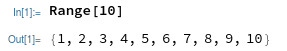
\includegraphics[width=0.7\linewidth]{pics/Range}
				\caption{Function Range[]}
				\label{fig:range}
			\end{figure}
			\paragraph{Reverse[] is a function to reverse the elements in a list}
			\begin{figure}[h!]
				\centering
				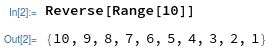
\includegraphics[width=0.7\linewidth]{pics/Reverse}
				\caption{Function Reverse[]}
				\label{fig:reverse}
			\end{figure}
			\paragraph{Use Join[] to join Lists together}
			\begin{figure}[h!]
				\centering
				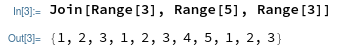
\includegraphics[width=0.7\linewidth]{pics/Join}
				\caption{Function Join[]}
				\label{fig:join}
			\end{figure}
		\section{Visualizing Lists}
			
		
		
		
			
			
			
			
				
				
\end{document}